\documentclass[11pt,a4paper]{article}
\usepackage{fontspec}
\usepackage[russian]{babel}
\usepackage[margin=2cm]{geometry}
\usepackage{booktabs,array,graphicx,hyperref,xcolor}
\usepackage{listings}
\usepackage{float}
\usepackage{indentfirst}
\setlength{\parindent}{1.25cm}
\lstset{
  basicstyle=\ttfamily\small,
  columns=fullflexible,
  breaklines=true,
  frame=single,
  showstringspaces=false,
}

% Computer Modern Unicode — загрузка по файлам
\setmainfont{cmunrm.otf}[
    BoldFont       = cmunbx.otf,
    ItalicFont     = cmunti.otf,
    BoldItalicFont = cmunbi.otf,
]
\setsansfont{cmunss.otf}[BoldFont = cmunsx.otf]
\setmonofont{cmuntt.otf}[BoldFont = cmuntb.otf]

\newcommand{\todo}[1]{\textcolor{red}{[#1]}}
\newcommand{\cmd}[1]{\texttt{#1}}
\newcommand{\shot}[3]{\begin{figure}[H]\centering
\includegraphics[width=#3\linewidth]{#1}\caption{#2}\end{figure}}
\title{Усиление защиты ядра Linux}

\author{Ростислав~Феськов}
\date{2 ноября 2026}
\begin{document}
\maketitle

\section{Введение}
По заданию нужно поиграться с различными настройками ядра Linux и проверить с помощью \cmd{kernel-hardening-checker}.

Ради интереса я решил взять сразу две виртуальные машины, которые запускались через QEMU — одну я запускал на Proxmox с архитектурой процессора AMD64, а вторую на macOS (с оболочкой UTM вокруг QEMU) с архитектурой ARM64 (или x86\_64 и AArch64, если говорить иначе). Поэтому обе машины работали на нативной архитектуре без эмуляции. Было интересно сравнить поведение ядер на двух разных архитектурах.


Виртуальные машины по характеристикам вышли вот такие:

\begin{tabular}{@{}lll@{}}
\toprule
Параметр & ВМ 1 (amd64) & ВМ 2 (aarch64)\\
\midrule
Имя хоста & int-6-amd64 & int-6-aarch64\\
Гипервизор & Proxmox (KVM) & UTM (Mac)\\
Архитектура & x86\_64 & arm64\\
Операционная система & Debian 13 (trixie) & Debian 13 (trixie)\\
Штатное ядро & 6.12.43+deb13 & 6.12.107+deb13\\
Собранные ядра & 6.12.113, 7.3.1 & 6.12.113, 7.3.1\\
Компилятор & GCC & GCC\\
Процессор (ядер) & 4 & 4\\
Оперативная память & 6 ГБ & 8 ГБ\\
Диск & 80 ГБ & 80 ГБ\\
\bottomrule
\end{tabular}

\section{Этапы}
Для удобста я поделил работу на этапы от s0 до s9 (state0-state9). От штатного ядра дистрибутива без изменений до новейшего ядра с харденингом.

\begin{tabular}{@{}ll@{}}
\toprule
Ступень & Что делаем\\
\midrule
s0 & Штатное состояние, без изменений\\
s1 & Ослабляем защиту (проверка, что тесты работают)\\
s2 & Включаем защиту через sysctl\\
s3 & Добавляем параметры загрузки ядра\\
s4 & Запрещаем userns, io\_uring и ptrace\\
s5 & Запрещаем загрузку модулей ядра\\
s6 & Включаем lockdown и прочие настройки\\
s7 & Собираем своё ядро 6.12.113 (\cmd{base})\\
s8 & Убираем лишний код из ядра (\cmd{hardening})\\
s9 & То же ядро версии 7.3.1\\
\bottomrule
\end{tabular}

\section{Результаты чекера}
На каждом этапе (кроме s1) запускался kernel-hardening-checker. Сводную таблицу результатов можно видеть ниже.

\begin{tabular}{@{}lrrrr@{}}
\toprule
Ступень & amd64 OK & amd64, \% & aarch64 OK & aarch64, \%\\
\midrule
s0 штатное & 190 & 51,9 & 179 & 55,6\\
s1 ослабление & \multicolumn{4}{c}{чекер не запускался (контроль тестов)}\\
s2 sysctl & 205 & 56,0 & 194 & 60,2\\
s3 cmdline & 232 & 63,4 & 201 & 62,4\\
s4 запреты & 235 & 64,2 & 204 & 63,4\\
s5 без модулей & 237 & 64,8 & 206 & 64,0\\
s6 lockdown & 239 & 65,3 & 208 & 64,6\\
s7 \cmd{base} & 240 & 65,6 & 209 & 64,9\\
s8 \cmd{hardening} & 335 & 91,5 & 290 & 90,1\\
s9 ядро 7.3.1 & 335 & 91,5 & 288 & 89,4\\
\bottomrule
\end{tabular}

\smallskip\noindent Проценты считались как OK/(OK+FAIL). Всего было 366 проверок на AMD64 и 322 на AArch64. Наибольший прирост дала сборка ядра с урезанным Kconfig (s7$\to$s8: $+95$ и $+81$ проверок соответственно), заметно больше, чем sysctl и командная строка вместе.

\section{Методика тестирования}
Для каждой ступени я запускал \cmd{./run\_tests.sh <ступень>} (например,
\cmd{s2\_sysctl}). Скрипт выполняет набор потенциально опасных команд. Результат OK означает, что команда
завершилась с кодом 0, то есть действие \emph{разрешено} (защиты нет). Любой
другой код возврата, включая превышение таймаута в 20~секунд, записывается как
BLOCKED (защита сработала либо действие не удалось). Первые 70 символов
вывода команды сохраняются рядом с результатом, чтобы понимать причину отказа
(\cmd{EPERM}, \cmd{ENOSYS}, \cmd{ENOSPC}, отсутствие файла).

Результаты пишутся в \cmd{\~{}/lab/results/<ступень>\_<архитектура>.tsv}, а рядом в
файл \cmd{.info} сохраняется состояние ядра (командная строка, режим lockdown и
значения девяти sysctl):\\
\cmd{dmesg\_restrict},\\
\cmd{kptr\_restrict},\\
\cmd{perf\_event\_paranoid},\\
\cmd{unprivileged\_bpf\_disabled},\\
\cmd{ptrace\_scope},\\
\cmd{max\_user\_namespaces},\\
\cmd{io\_uring\_disabled},\\
\cmd{modules\_disabled},\\
\cmd{kexec\_load\_disabled}.\\
Это подтверждает, при каких настройках получены
результаты. Скрипт \cmd{matrix.py} собирает все \cmd{.tsv}-файлы текущей архитектуры
в сводную таблицу <<тест~$\times$~ступень>>. Тесты выполнялись одним и тем же
скриптом на обеих ВМ.

\begin{tabular}{@{}p{3cm}p{8cm}p{3.8cm}@{}}
\toprule
Тест & Команда & Чем закрывается\\
\midrule
\cmd{dmesg\_user} & \cmd{dmesg} от обычного пользователя & \cmd{dmesg\_restrict}\\
\cmd{kallsyms\_root} & \cmd{sudo grep} находит \cmd{\_text} в \cmd{/proc/kallsyms} с ненулевым адресом & \cmd{kptr\_restrict}, \cmd{KALLSYMS=n}\\
\cmd{perf\_user} & \cmd{perf stat -e task-clock true} & \cmd{perf\_event\_paranoid}\\
\cmd{bpf\_user} & программа \cmd{bpf\_demo} (на~C) делает вызов \cmd{bpf} & \cmd{unprivileged\_bpf\_disabled}\\
\cmd{ptrace\_child} & программа \cmd{ptrace\_demo} (на~C): \cmd{ptrace(ATTACH)} к дочернему процессу & \cmd{yama.ptrace\_scope}\\
\cmd{userns} & \cmd{unshare -Ur true} & \cmd{max\_user\_namespaces}, \cmd{USER\_NS=n}\\
\cmd{bwrap} & \cmd{bwrap --unshare-user --ro-bind / / true} (требует userns) & то же\\
\cmd{io\_uring} & системный вызов 425 (\cmd{io\_uring\_setup}) через \cmd{ctypes} & \cmd{io\_uring\_disabled}, \cmd{IO\_URING=n}\\
\cmd{modprobe} & \cmd{modprobe dummy} и выгрузка & \cmd{modules\_disabled}\\
\cmd{kexec\_load} & \cmd{kexec -l} текущего ядра, затем \cmd{kexec -u} & lockdown, \cmd{KEXEC=n}\\
\cmd{proc\_kcore} & \cmd{sudo head -c 4 /proc/kcore} & lockdown, \cmd{PROC\_KCORE=n}\\
\cmd{ctl\_dns} & \cmd{getent hosts deb.debian.org} & --- контроль\\
\cmd{ctl\_https} & \cmd{curl} к \cmd{https://deb.debian.org}, ожидается код 200 & --- контроль\\
\cmd{ctl\_systemd} & \cmd{systemctl is-system-running} равно \cmd{running} или \cmd{degraded} & --- контроль\\
\bottomrule
\end{tabular}

\smallskip\noindent Тесты \cmd{ctl\_*} не должны переходить в BLOCKED, иначе запрет сломал саму систему. Ниже представлены скриншоты со сводной матрицей тестов по каждому из этапов.

\begin{figure}[H]\centering
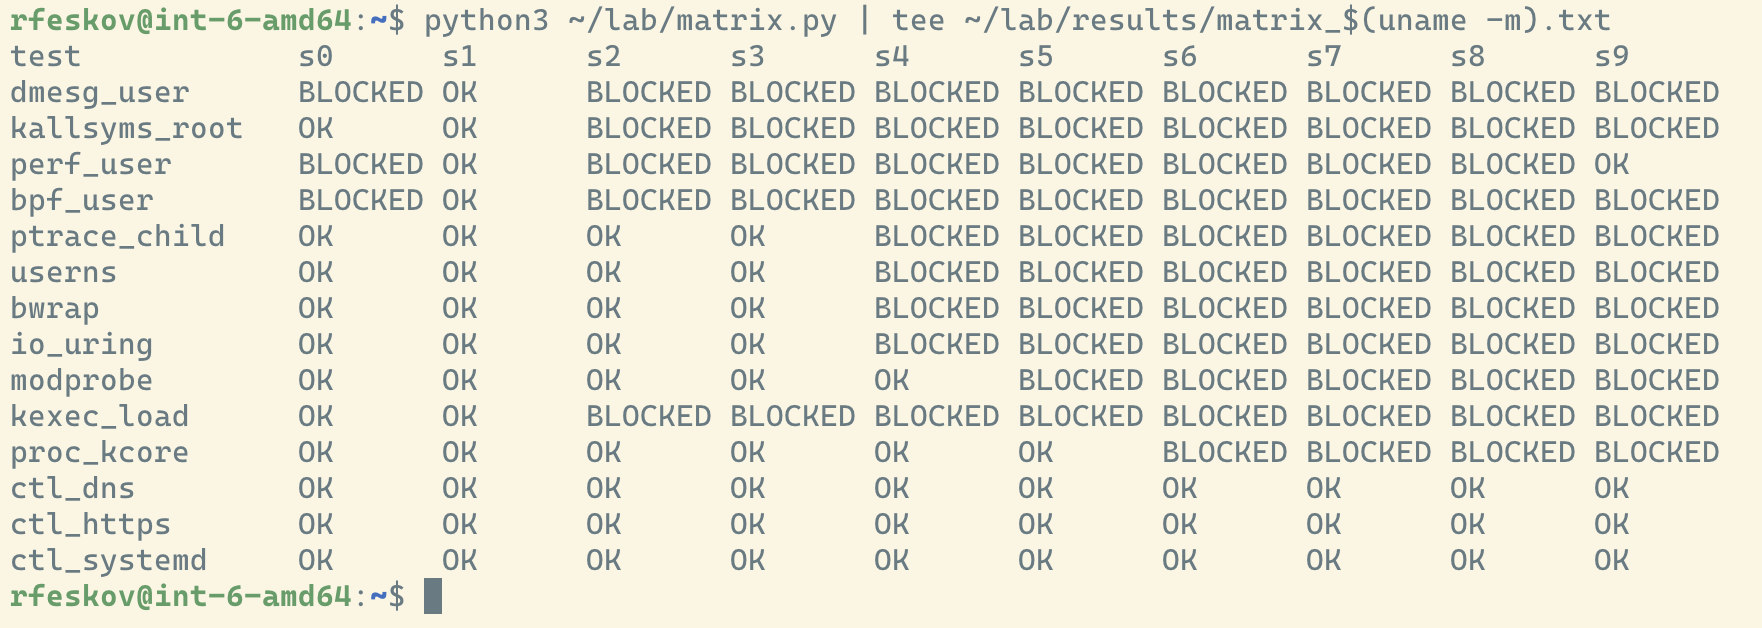
\includegraphics[width=\linewidth]{matrix-amd.png}
\caption{Сводная матрица тестов, amd64}
\end{figure}
\begin{figure}[H]\centering
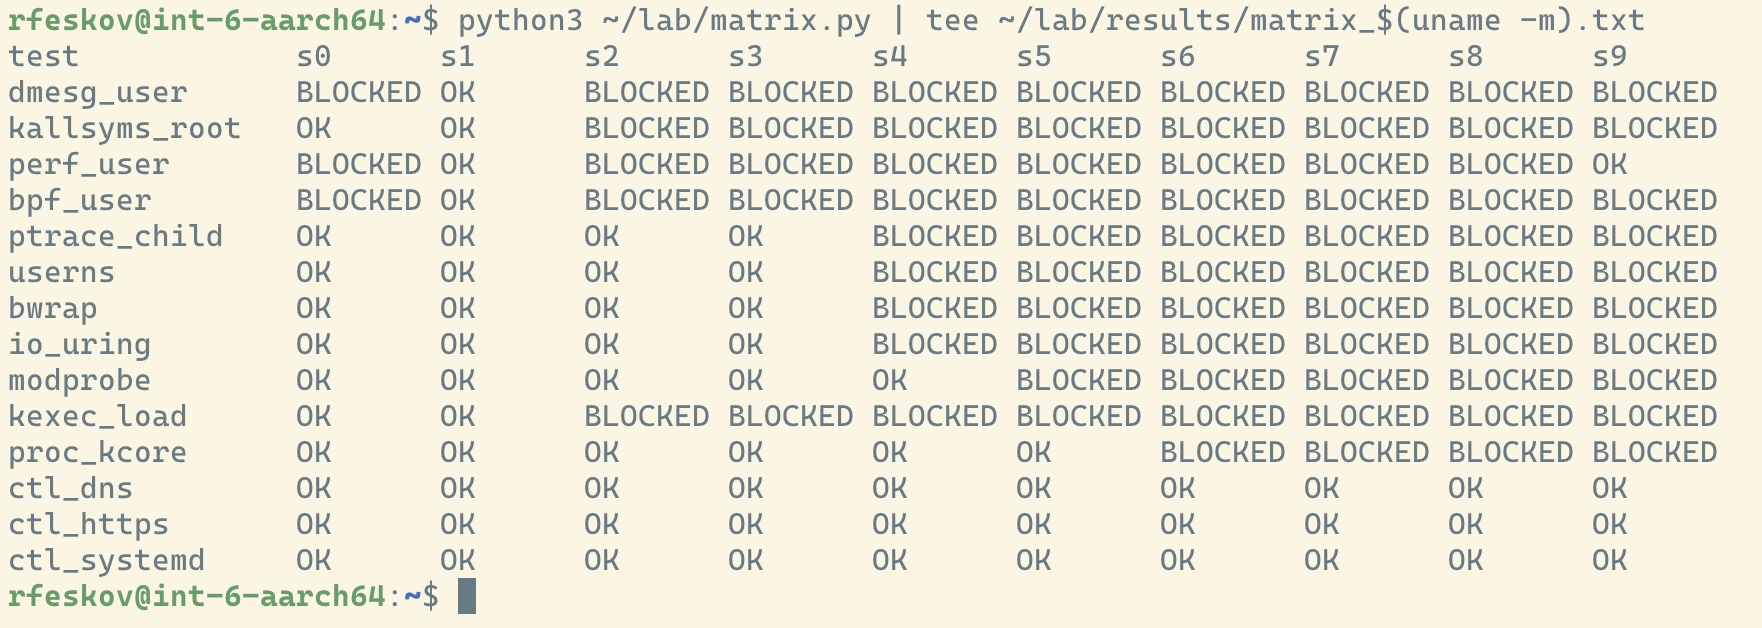
\includegraphics[width=\linewidth]{matrix-aarch.png}
\caption{Сводная матрица тестов, aarch64}
\end{figure}

Ступень s1 служит контролем, показывающим, что защитные тесты способны давать OK.

Ниже представлен листинг кода тестов и создания матрицы.

\lstinputlisting[caption={Скрипт запуска тестов \cmd{run\_tests.sh}},label={lst:run}]{run_tests.sh}
\lstinputlisting[language=Python,caption={Сводка результатов \cmd{matrix.py}},label={lst:matrix}]{matrix.py}

\subsection*{Ограничения методики}
BLOCKED объединяет все причины неудачи (запрет политикой, отсутствие кода,
таймаут), поэтому причину нужно читать из сохранённого вывода. К тому же, тесты проверяют
по одному способу обойти защиту, а не все возможные. Тест \cmd{userns} и \cmd{bwrap}
зависят друг от друга, так как \cmd{bwrap} использует пространство имён пользователя.

\section{Поведенческие тесты}
Матрицы тестов для обеих машин показаны выше, и они получились одинаковыми. Тесты \cmd{ctl\_*} везде остались OK, значит система работоспособна.

На s0 Debian сам закрывает \cmd{dmesg}, \cmd{perf} и \cmd{bpf} для обычного пользователя.

На s1 я это ослабил, и все три теста стали OK, так я проверил, что тесты вообще работают.

На s2 после sysctl закрылись \cmd{kallsyms\_root} и \cmd{kexec\_load}.

На s3 в тестах ничего не поменялось, хотя чекер вырос сразу на 27 проверок на amd64.

На s4 закрылись \cmd{ptrace\_child}, \cmd{userns}, \cmd{bwrap} и \cmd{io\_uring}.

На s5 закрылся \cmd{modprobe}, потому что загрузка модулей стала запрещена.

На s6 \cmd{proc\_kcore}, это сделал режим lockdown.

Интересно, что при \cmd{max\_user\_namespaces=0} тест \cmd{userns} выдал не <<Operation not permitted>>, а <<No space left on device>>.
\begin{lstlisting}[numbers=none]
userns   BLOCKED  unshare: unshare failed: No space left on device
bwrap    BLOCKED  bwrap: Creating new namespace failed: nesting depth or /proc/sys/user/
\end{lstlisting}

Между s7 и s8 матрица не изменилась, а чекер вырос на 95 проверок на amd64 и на 81 на aarch64. Запреты остались теми же, но теперь код в принципе вырезан из ядра, и снять их командой уже нельзя.

На s8 файлов \cmd{/proc/kallsyms} и \cmd{/proc/kcore} просто нет. Ошибка \cmd{userns} тоже стала другой: сначала \cmd{ENOSPC}, потом \cmd{EPERM} на 6.12.113 и \cmd{EINVAL} на 7.3.1.

На 7.3.1 тест \cmd{perf\_user} снова стал OK. Значение \cmd{perf\_event\_paranoid} при этом равно 3, и на 6.12.113 с ним всё работало. Причину я не искал, но надёжнее закрывать \cmd{perf} отключением \cmd{PERF\_EVENTS} при сборке.

\begin{tabular}{@{}lll@{}}
\toprule
Тест & s8 (6.12.113) & s9 (7.3.1)\\
\midrule
\cmd{perf\_user} & BLOCKED & OK\\
\cmd{userns} & \cmd{EPERM} & \cmd{EINVAL}\\
остальные & BLOCKED & BLOCKED\\
\bottomrule
\end{tabular}

\section{Остаточные FAIL}
После s8 чекер оставил 31 FAIL на amd64 и 32 на aarch64. Почти все они объясняются просто.

\begin{itemize}
\item Нужен Clang, а ядро собрано GCC. Это \cmd{CFI\_CLANG}, параметр \cmd{cfi}, \cmd{ARM64\_BTI\_KERNEL} и \cmd{SHADOW\_CALL\_STACK}.
\item Нужны плагины GCC, которых в системе нет. Это \cmd{RANDSTRUCT\_FULL}, \cmd{GCC\_PLUGIN\_LATENT\_ENTROPY} и \cmd{KSTACK\_ERASE}.
\item Нет в железе виртуалок. Это \cmd{KASAN\_HW\_TAGS}, \cmd{ARM64\_GCS} и \cmd{iommu=force}.
\item Остались от конфига Debian \cmd{MODULES}, \cmd{BPF\_SYSCALL}, \cmd{KCMP}, \cmd{VT}, \cmd{FB}, \cmd{TLS} и \cmd{IP\_SCTP}.
\item Параметр \cmd{nosmt} ложно считается FAIL, он задан внутри \cmd{mitigations=auto,nosmt}, а чекер ищет его отдельно.
\item Я не включал \cmd{UBSAN\_*}, \cmd{WERROR}, \cmd{STATIC\_USERMODEHELPER} и \cmd{vm.mmap\_rnd\_bits}.
\end{itemize}

\section{Сравнение 6.12.113 и 7.3.1}
Инрересно, что при смене версии ядра с 6 до самого последнего релиза 7, почти ничего не изменилось. Конфиг я перенёс как есть через \cmd{make olddefconfig}.

\begin{tabular}{@{}lll@{}}
\toprule
Опция & amd64 & aarch64\\
\midrule
\cmd{HARDENED\_USERCOPY\_DEFAULT\_ON} & FAIL $\to$ OK & FAIL $\to$ OK\\
\cmd{ARM64\_GCS} & -- & FAIL $\to$ OK\\
\cmd{RANDOM\_KMALLOC\_CACHES} & OK $\to$ FAIL & OK $\to$ FAIL\\
\cmd{ARM64\_PAN}, \cmd{RODATA\_FULL\_DEFAULT\_ENABLED}, \cmd{rodata} & -- & OK $\to$ FAIL\\
\bottomrule
\end{tabular}

\smallskip\noindent В итоге на amd64 осталось 335 пройденных проверок, а на aarch64 стало 288 вместо 290. Выходит, что версия ядра сама по себе защиту не повышает, всё решает конфигурация.

\section{Трудности сборки}
На aarch64 сборка 7.3.1 упала в драйвере Marvell OcteonTX2, потому что ему нужен \cmd{CONFIG\_DEBUG\_FS}, а у меня он выключен. Драйвер в виртуалке не нужен, поэтому я его просто отключил.

Пакеты получили двойное имя \cmd{7.3.1-hardening-hardening}, потому что суффикс был и в \cmd{.config}, и в команде сборки. На работу ядра это не влияет. Из-за обрывов SSH сборку я запускал в \cmd{tmux}.

\section{Выводы}
Больше всего защиты дало удаление кода из ядра, а не настройки. Переход от s7 к s8 добавил 95 проверок на amd64 и 81 на aarch64, а все sysctl и параметры загрузки вместе дали 50 и 30.

Тесты показали, что запреты работают и система остаётся рабочей. Новое ядро 7.3.1 лучше не стало, а \cmd{perf\_event\_paranoid=3} на нём перестал работать.

\section*{Приложение}

\subsection*{Стенд}
\shot{vm-amd-info.png}{Характеристики ВМ amd64 (KVM, Intel N150, 4 ядра, Debian 13)}{0.9}
\shot{vm-aarch-info.png}{Характеристики ВМ aarch64 (QEMU на Mac, 4 ядра, Debian 13)}{0.9}
\shot{vm-amd-res.png}{Память, диск и загрузка UEFI на amd64, флаги процессора}{0.9}
\shot{vm-aarch-res.png}{Память, диск и загрузка UEFI на aarch64}{0.9}

\subsection*{Ступень s0, штатное состояние}
\shot{s0-amd-checker.png}{Итог чекера на s0, amd64 (190 OK, 176 FAIL)}{0.7}
\shot{s0-aarch-checker.png}{Итог чекера на s0, aarch64 (179 OK, 143 FAIL)}{0.7}
\shot{s0-amd-rec.png}{Список проверок чекера для x86\_64 (файл rec\_x86\_64.txt)}{0.8}
\shot{s0-aarch-rec.png}{Список проверок чекера для ARM64 (файл rec\_arm64.txt)}{0.8}

\subsection*{Ступени s0 и s1, тесты}
\shot{s01-amd-tests.png}{Тесты на s0 и s1, amd64}{0.85}
\shot{s01-aarch-tests.png}{Тесты на s0 и s1, aarch64}{0.85}

\subsection*{Ступень s2, sysctl}
\shot{s2-amd.png}{Значения sysctl и тесты на s2, amd64}{0.9}
\shot{s2-aarch.png}{Значения sysctl и тесты на s2, aarch64}{0.9}

\subsection*{Ступень s3, параметры загрузки}
\shot{s3-amd-grub.png}{Параметры ядра в редакторе GRUB, amd64}{0.8}
\shot{s3-aarch-grub.png}{Параметры ядра в редакторе GRUB, aarch64}{0.7}

\subsection*{Ступень s7, собственное ядро base}
\shot{s7-amd-build.png}{Сборка и установка ядра base, amd64 (около 88 минут)}{0.8}
\shot{s7-aarch-build.png}{Сборка и установка ядра base, aarch64 (около 35 минут)}{0.8}
\shot{s7-amd-tests.png}{Тесты и чекер на ядре base, amd64 (240 OK, 126 FAIL)}{0.85}
\shot{s7-aarch-tests.png}{Тесты и чекер на ядре base, aarch64 (209 OK, 113 FAIL)}{0.85}

\subsection*{Ступень s8, ядро hardening}
\shot{s8-amd.png}{Тесты и чекер на ядре hardening, amd64 (335 OK, 31 FAIL)}{0.85}
\shot{s8-aarch.png}{Тесты и чекер на ядре hardening, aarch64 (290 OK, 32 FAIL)}{0.85}
\end{document}
